\chapter{Particle Net Simplifications}


\section{Simpler Architectures}

\subsection{The full network}

\begin{figure}[H]
    \centering
    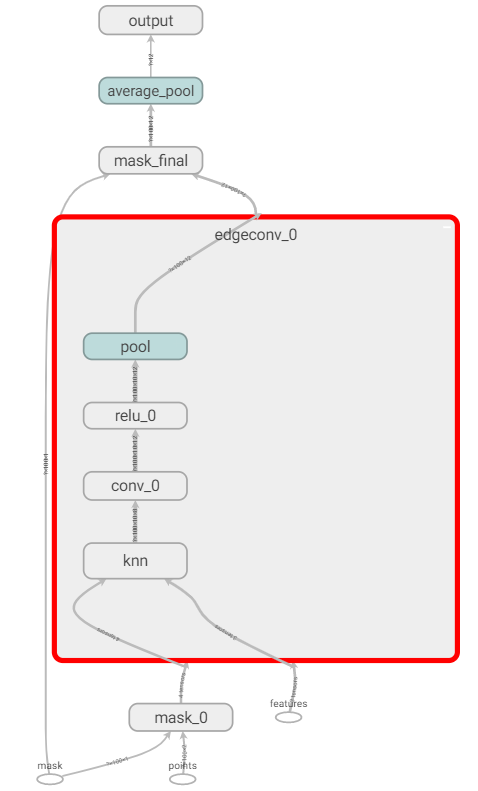
\includegraphics[width=0.4\linewidth]{img/simplify-particle-net/network.png}
    \caption{Neural Network Graph Visualization}
\end{figure}



\section{Distribution of Parameters}

\subsection{Weight Histograms}

\begin{figure}[H]
    \centering
    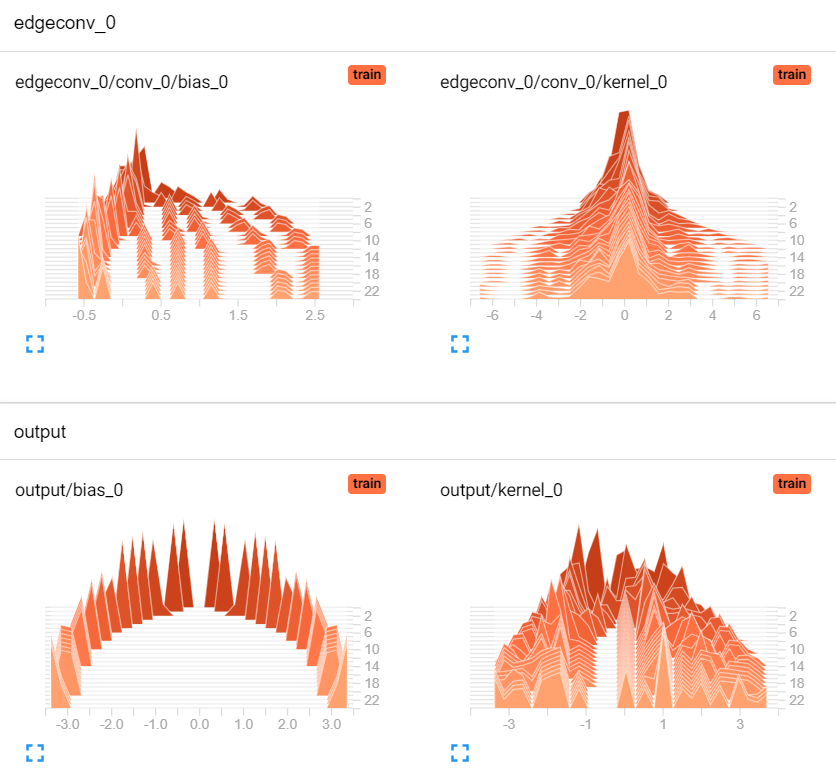
\includegraphics[width=0.8\linewidth]{img/simplify-particle-net/histograms.png}
    \caption{TensorBoard Histograms}
\end{figure}

We see that our biases are very important, and the the network is learning quite something. All layers are important.

\subsection{Weight Distribution}

\begin{figure}[H]
    \centering
    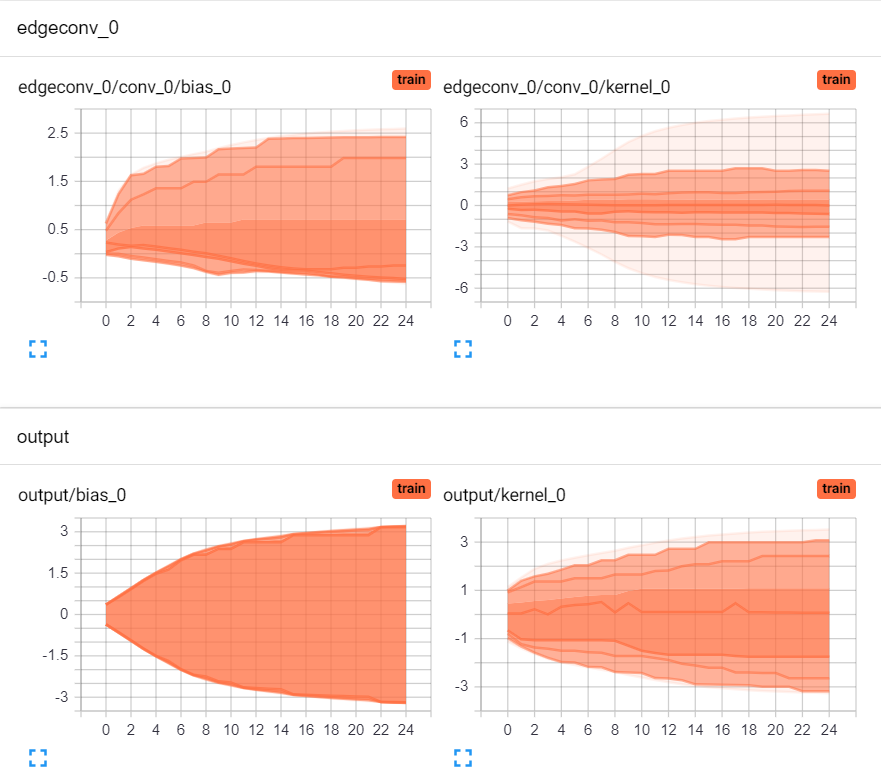
\includegraphics[width=0.8\linewidth]{img/simplify-particle-net/distributions.png}
    \caption{TensorBoard Histograms}
\end{figure}


\subsection{Feature Polynomials}

\begin{tabular}{|c|c|c|c|c|c|c|c|c|}
    \hline
    .           & \textbf{Hub-$\eta$} & \textbf{Hub-$\phi$} & \textbf{Hub-$p_t$} & \textbf{Hub-$E$} & \textbf{Rel-$\eta$} & \textbf{Rel-$\phi$} & \textbf{Rel-$p_t$} & \textbf{Rel-$E$} \\
    \hline
    \textbf{00} & 1.39279             & 2.95816             & 0.47035            & 0.15665          & 2.13112             & 2.54264             & -1.58122           & -1.02798         \\
    \textbf{01} & -1.56491            & -2.16750            & 0.32590            & 0.38175          & 0.46990             & -1.77234            & -1.51412           & -1.93057         \\
    \textbf{02} & 1.10430             & 2.35467             & 0.66460            & 0.03594          & 2.26508             & 1.87872             & -1.13675           & -1.95035         \\
    \textbf{03} & -3.58598            & 6.64981             & -0.04281           & 0.11523          & 0.28928             & 0.05610             & 0.43508            & -0.46872         \\
    \textbf{04} & 5.51387             & -3.83200            & -0.12499           & 0.62469          & 4.76349             & -3.50846            & -0.96857           & -0.62145         \\
    \textbf{05} & -6.26354            & -4.09571            & 0.32543            & -0.21911         & -0.16259            & -0.11651            & -0.15742           & 0.11673          \\
    \textbf{06} & -1.61074            & 0.18924             & -0.50111           & 0.71576          & 1.02103             & -0.94762            & 0.00520            & -0.64432         \\
    \textbf{07} & -1.36603            & -0.10369            & 0.63901            & 0.74640          & 2.91987             & 1.39712             & -0.19567           & 1.04621          \\
    \textbf{08} & -1.03466            & 0.14385             & -0.61606           & -0.28012         & 1.07867             & -0.29486            & 0.20878            & 0.05523          \\
    \textbf{09} & -0.87198            & -2.81173            & 0.55644            & 0.16556          & 0.96585             & -2.10658            & -1.37593           & -2.11623         \\
    \textbf{10} & -0.65812            & 0.37103             & 0.27153            & 0.89163          & -1.76185            & 2.72242             & -0.35294           & -0.27357         \\
    \textbf{11} & -1.14922            & 0.11895             & -1.00611           & 0.25360          & 1.05348             & -0.16677            & 0.58487            & -0.37585         \\
    \hline
\end{tabular}

We train a dataset on these 12 transformed features. The relative weights of the feature follow here, the following are our notes:
\begin{itemize}
    \item Decision Tree with max-depth 8 gives accuarcy of 81.67\% when just trained on faetures 2 and 11.
    \item Decision Tree with max-depth 8 gives accuarcy of 85.00\% when trained on features 2, 11, 9, 3, 1.
\end{itemize}
\begin{figure}[H]
    \centering
    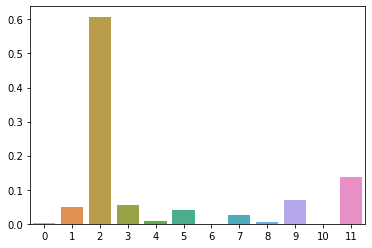
\includegraphics[width=0.8\linewidth]{img/simplify-particle-net/feature-importances.png}
    \caption{Relative Feature importances}
\end{figure}
